%%%%%%%%%%%%%%%%%%%%%%%%%%%%%%%%%%%%%%
% P R O F I L E
%%%%%%%%%%%%%%%%%%%%%%%%%%%%%%%%%%%%%%
\begin{facts}
    % \adjustbox{valign=t}{
    % \begin{tikzpicture}[scale=0.85]
    %     \filldraw[fill=imageborder] (0,0) circle (2.7cm);
    %     \clip (0,0) circle (2.5cm);
    %     \node[anchor=center] at (0, 0.25) {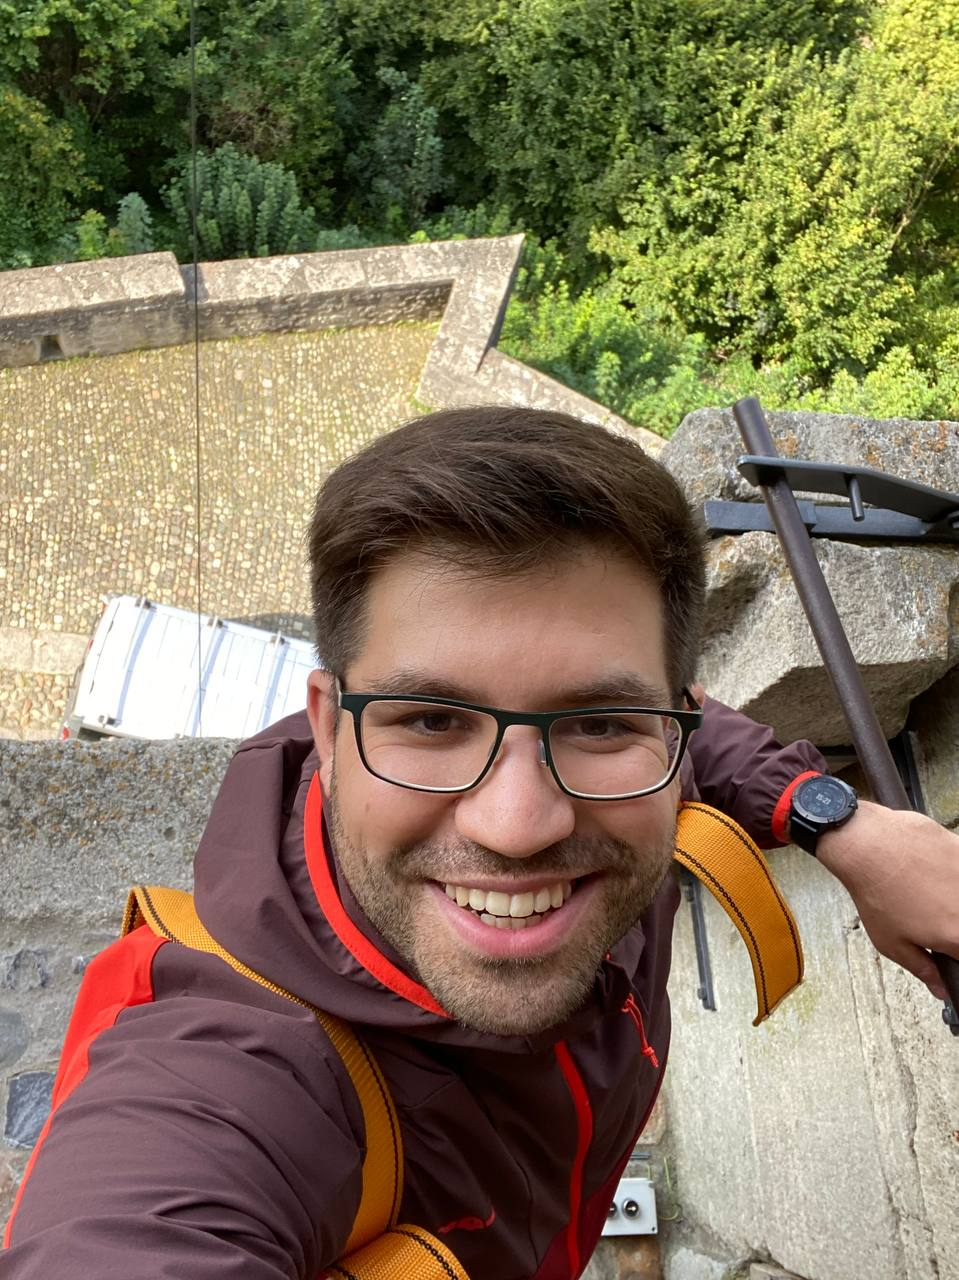
\includegraphics[width=4.5cm]{images/me}}; 
    %     %adjust this coordinate to move image
    % \end{tikzpicture}
    % }
    % \sectionsep
    \section{Noah Hüsser}
    % Nationality: Swiss\\
    % Date of Birth: 12th January 1991
    \sectionsep
    
    \subsubsection{Contact}
    noah@huesser.dev\\
    +41 79 960 7130\\
    \href{https://github.com/Yatekii}{https://github.com/Yatekii}\par
    % \vspace{\baselineskip}
    % Ammerswilerstrasse 31F\\
    % 5600 Lenzburg\\
    % Switzerland
    \sectionsep
    
    %%%%%%%%%%%%%%%%%%%%%%%%%%%%%%%%%%%%%%
    % S K I L L S
    %%%%%%%%%%%%%%%%%%%%%%%%%%%%%%%%%%%%%%
    \subsubsection{Professional Skills}
    Embedded Engineering\\
    Software Development\\
    SRE\\
    Project Management
    \sectionsep

    \subsubsection{Engineering Tools}
    Linux/Unix, Bash\\
    Docker, K8S, Nomad, Terraform\\
    Gitlab CI, Github Actions\\
    Splunk, Grafana, ElasticSearch\\
    Jupyter, Scipy, Numpy, Pandas\\
    Kafka, Redis, Postgres\\
    Git
    \sectionsep

    \subsubsection{Programming}
    \describe{frequently used}\\
    Rust, TypeScript, Python,\\
    Dart, C, SQL
    \sectionsep
    
    \describe{used in the past}\\
    Bash, C\#, C++, Java, LaTeX, Tcl, PHP, VHDL, VB.NET
    \sectionsep
    
    \subsubsection{Languages}
    German \describe{mother tongue}\\
    English \describe{fluent}\\
    French \describe{experienced}\\
    Spanish \describe{basic}\\
    Polish and Arabic \describe{learning}
    \sectionsep
    
    \subsubsection{Activities}
    Programming, Electronics,\\
    Kite Surfing, Ju Jitsu, \\
    Running
    \sectionsep
    
    \subsubsection{References}
    on request
    
    \sectionsep
    Last updated \today.
    
    \end{facts}%
    \begin{timeline}
    
    %%%%%%%%%%%%%%%%%%%%%%%%%%%%%%%%%%%%%%
    %     EXPERIENCE
    %%%%%%%%%%%%%%%%%%%%%%%%%%%%%%%%%%%%%%
    
    \subsection{Practical Experience}

    \subsubsection{Lead Embedded and Electrical Engineer - SG-1}
    \meta{Helsing}{June 2025}{present}{Zürich}
    \textbf{Firmware tech lead of the UUV SG-1} in a team of 4. Building everything from the ground up in Rust.
    \begin{tightemize}
        \item Bootstrapped the architecture from the ground up enabling rapid testing and confident deployments.
        \item Overhauled the electrical design to address electrical and manufacturing issues cutting iteration times by entire days per feature.
        \item Bootstrapped the electrical RND lab in the factory.
        \item Introduction of new members to embedded best practices.
    \end{tightemize}
    \sectionsep

    \subsubsection{Senior Software Engineer - Rust Backend}
    \meta{Kraken}{December 2021}{February 2025}{Zürich}
    \textbf{Maintainer of the microservice} routing and access controlling all internal RPC.
    Focus on service stability, performance, technology choices and DX.
    \begin{tightemize}
        \item Managing all releases to \textbf{10 million users}.
        \item Work on \textbf{latency, operations and CI improvements} as well as \textbf{new features}.
        \item \textbf{Onboarded 5 new team members} into engineering workflows.
        \item \textbf{On call} incident and vulnerability response.
    \end{tightemize}
    \sectionsep

    \subsubsection{Co-Founder \& Lead Software Engineer - Python, Dart, C}
    \meta{Siglis (part-time)}{August 2020}{August 2021}{Zürich}
    Developed a smart switch with \textbf{Zigbee and Bluetooth} communication (\href{https://zigfred.ch}{zigfred.ch}).
    \begin{tightemize}
        \item Built the \textbf{manufacturing pipeline \& oversight} in \textbf{Python} and \textbf{TypeScript}.
        \item Built a \textbf{mobile app} to configure and control switches - in \textbf{Dart}. 
        \item Implemented automated \textbf{DFU} including bootloader, transfer via bluetooth and automatic rollbacks - in \textbf{C}.
    \end{tightemize}
    \sectionsep
    
    \subsubsection{Co-Founder \& Lead Software Engineer - Rust, C, Python, C\#}
    \meta{Technokrat}{May 2017}{September 2021}{Zürich}
    Built software for \textbf{embedded devices}, cloud services and web applications.
    \begin{tightemize}
        \item Simulated variations of coil arrays for wireless power transfer in \textbf{Python} and \textbf{Rust}, which resulted in \textbf{two patents}.
        \item Designed a system to \textbf{assign bushings} to different curing vessels and plan the curing process.
        \item Designed an EVSE controller - in \textbf{Rust} - for J1772 based charging deployed to \textbf{thousands of EV charging stations}.
    \end{tightemize}
    \sectionsep

    \subsubsection{Senior Software Engineer - C\#, VB.Net}
    \meta{ABB}{Jul 2016}{March 2018}{Zürich}
    \begin{tightemize}
        \item Created an \textbf{MES} to supervise the manufacturing of \textbf{7000 bushings/year} (backend in \textbf{C\#} and \textbf{SQL}, frontend in \textbf{TypeScript}).
        \item Developed a UI CAD tool to dimension bushings (C\#, VB.Net, WPF UI).
        \item Larger scale data analysis in \textbf{Python}.
    \end{tightemize}
    \sectionsep

    % \subsubsection{Nexus Telecom}
    % \meta{Low Level C Programmer}{Mai 2014}{Mai 2015}{Zürich}
    % Porting the core C library from a strictly 32 bit architecture to 32/64 bit.
    % \sectionsep

    %%%%%%%%%%%%%%%%%%%%%%%%%%%%%%%%%%%%%%
    %     PUBLICATIONS
    %%%%%%%%%%%%%%%%%%%%%%%%%%%%%%%%%%%%%%
    
    \subsection{Publications and Open Source}

    \subsubsection{probe-rs embedded toolchain}
    \meta{Project Lead}{Mar 2019}{present}{\href{https://probe.rs}{probe.rs}}
    The toolkit allows to control \textbf{embedded ARM and RISC-V MCUs} to be controlled from a host.
    The project offers:
    \begin{tightemize}
    \item a library to \textbf{control targets from host code}
    \item \textbf{CLI tools} to flash and log data from targets
    \item A \textbf{VSCode debugger plugin}
    \end{tightemize}
    \sectionsep
    
    % \subsubsection{FPGA Based Spectrum Analyzer}
    % \meta{Bachelor Thesis at FHNW}{Mar 2017}{Aug 2017}{Windisch}
    % The tasks included, but were not limited to, the implementation of:
    % \begin{tightemize}
    % \item \textbf{CIC/FIR-filter}-chains for data decimation
    % \item A server to transmit data via \textbf{WebSockets} on an \textbf{embedded Linux}
    % \item A GUI to retrieve data over WebSockets, transform and display it (\textbf{JavaScript})
    % \end{tightemize}
    % \sectionsep
    
    % \subsubsection{FPGA Based Oscilloscope}
    % \meta{Group Thesis at ETH Zürich}{Sep 2015}{Dec 2015}{Zürich}
    % The tasks included, but were not limited to, the implementation of:
    % \begin{tightemize}
    % \item Recursive trigger logic to detect special signal patterns (VHDL)
    % \item Kernel module for data reading and processing on an ARM Core A9 (C)
    % \item GUI to retrieve data over TCP/IP, filter and display it (C++, Python, Qt5)
    % \end{tightemize}
    % \sectionsep

    % %%%%%%%%%%%%%%%%%%%%%%%%%%%%%%%%%%%%%%
    % %     VOLUNTEER EXPERIENCE
    % %%%%%%%%%%%%%%%%%%%%%%%%%%%%%%%%%%%%%%
    
    % \subsection{Volunteer Experience}
    
    % \subsubsection{Ju Jitsu Club Aarau}
    % \meta{Treasurer}{Apr 2019}{Apr 2023}{Aarau}
    % \sectionsep

    % \subsubsection{Bastli, Students Lab, ETH Zurich}
    % \meta{President}{Feb 2016}{Oct 2016}{Zürich}
    % \meta{Treasurer}{Feb 2015}{Feb 2016}{Zürich}
    % \sectionsep

    %%%%%%%%%%%%%%%%%%%%%%%%%%%%%%%%%%%%%%
    %     EDUCATION
    %%%%%%%%%%%%%%%%%%%%%%%%%%%%%%%%%%%%%%
    
    \subsection{Education}
    
    \subsubsubsection{FHNW Brugg-Windisch}
    \meta{BSc in EE and IT}{2016}{2017}{Windisch}
    
    \subsubsubsection{ETH Zürich}
    \meta{BSc in EE and IT (unfinished)}{Sep 2013}{Feb 2016}{Zürich}

    \end{timeline}%